\documentclass[border=6pt]{standalone}
\usepackage{tikz}
\usepackage{pgfplots}
\pgfplotsset{compat=1.18}
\usetikzlibrary{arrows.meta,positioning,shapes.geometric,fit,backgrounds,calc,decorations.pathreplacing,patterns}
\usetikzlibrary{pgfplots.groupplots}
\tikzset{
  blk/.style={rectangle, rounded corners=2pt, draw=black!70, thick, fill=blue!6,
              minimum height=8mm, minimum width=20mm, align=center, font=\small},
  io/.style={rectangle, rounded corners=6pt, draw=black!70, thick, fill=green!8,
             minimum height=8mm, align=center, font=\small},
  proc/.style={rectangle, draw=black!70, thick, fill=orange!10, minimum height=8mm,
               align=center, font=\small},
  dec/.style={diamond, aspect=2, draw=black!70, thick, fill=yellow!15, align=center, font=\footnotesize},
  warnbox/.style={rectangle, rounded corners=2pt, draw=red!60!black, thick, fill=red!7,
                  minimum height=8mm, align=center, font=\small},
  oklbox/.style={rectangle, rounded corners=2pt, draw=green!45!black, thick, fill=green!8,
                 minimum height=8mm, align=center, font=\small},
  ar/.style={-{Latex[length=2mm]}, thick},
  arl/.style={-{Latex[length=2mm]}, thick, dashed, draw=black!55},
  lbl/.style={font=\footnotesize\itshape, text=black!60},
}
\definecolor{good}{RGB}{34,139,34}
\definecolor{bad}{RGB}{178,34,34}
\definecolor{warn}{RGB}{218,165,32}
\definecolor{pesblue}{RGB}{0,45,98}
\definecolor{complete}{RGB}{30,125,79}
\definecolor{partial}{RGB}{176,106,0}
\definecolor{blocked}{RGB}{166,43,43}
\begin{document}
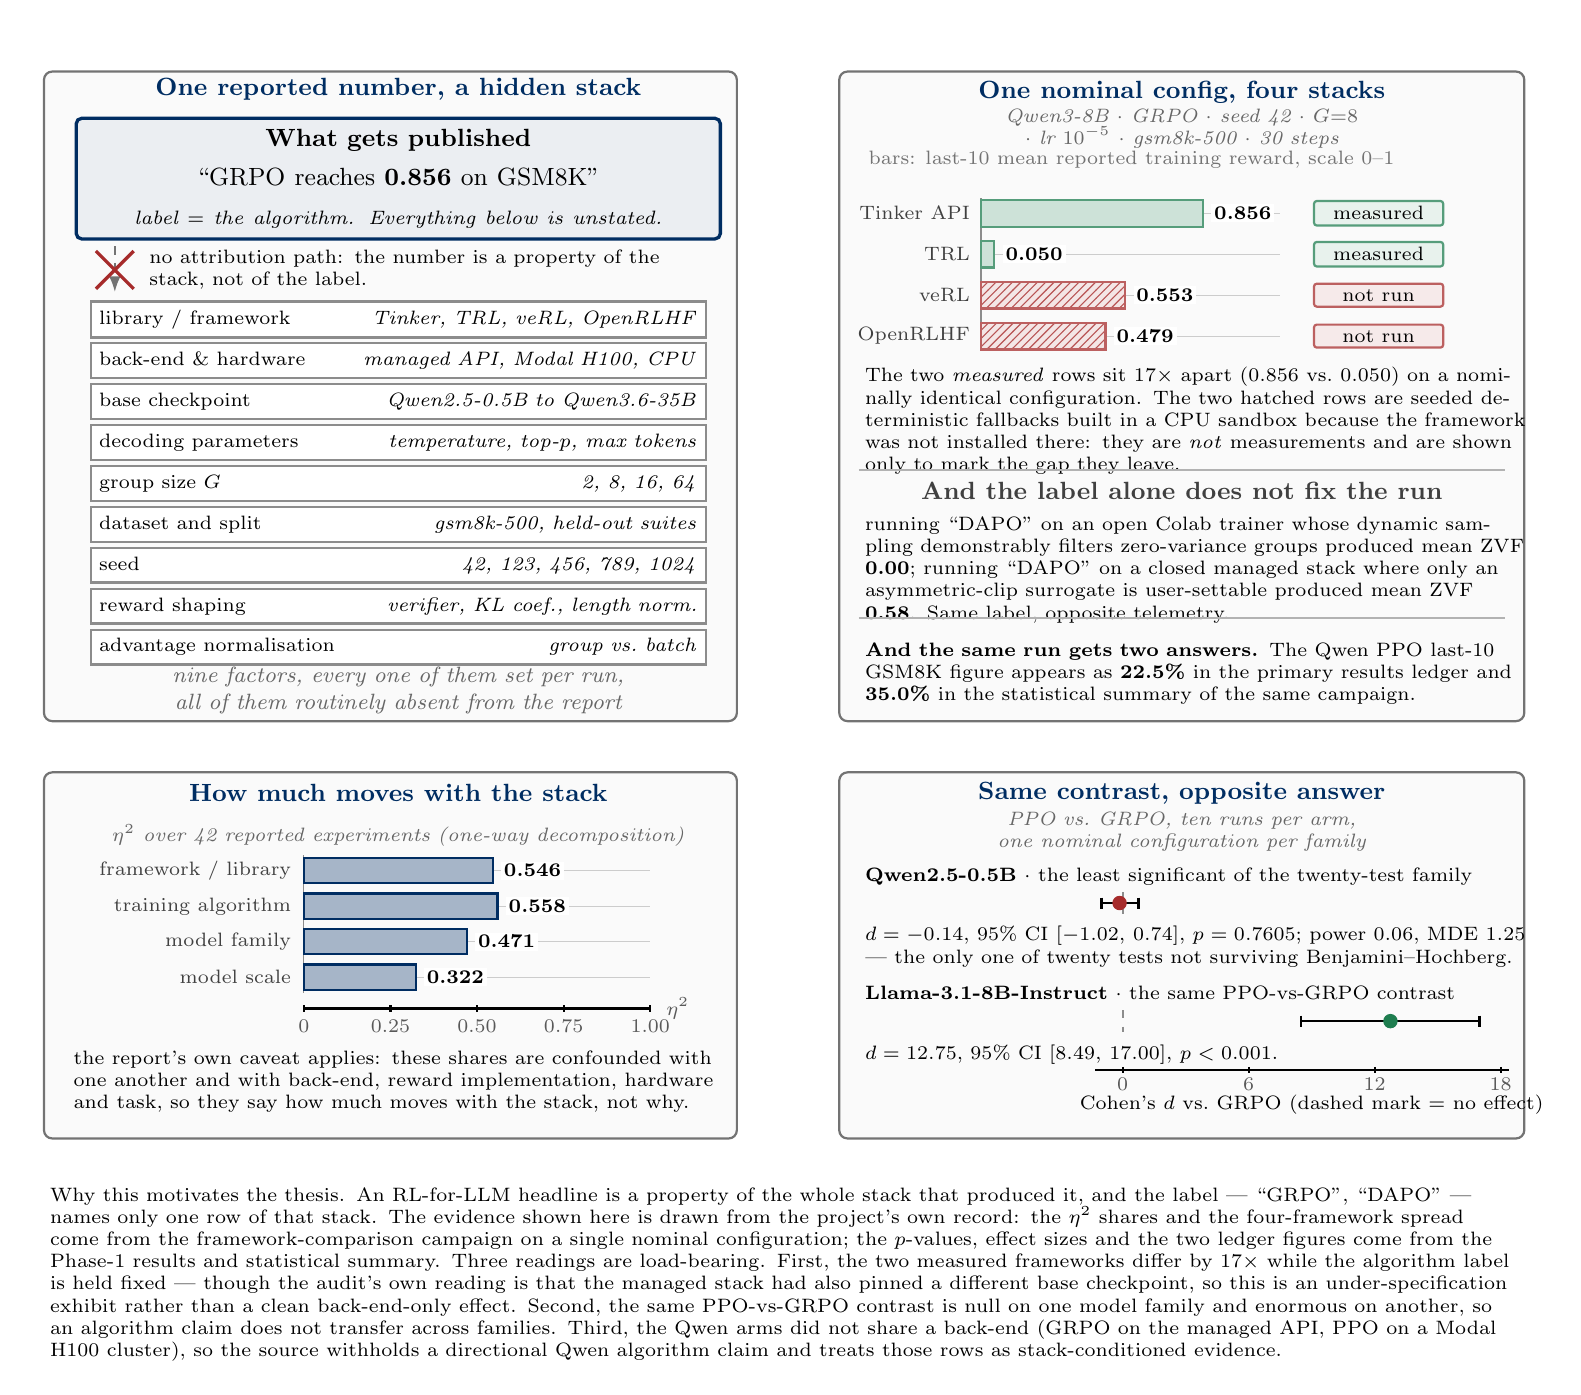
\begin{tikzpicture}[x=1cm,y=1cm,
  panel/.style={draw=black!55, thick, rounded corners=3pt, fill=black!2},
  pnlw/.style={draw=warn!70!black, thick, rounded corners=3pt, fill=warn!4},
  ptitle/.style={font=\small\bfseries, text=pesblue, align=center, inner sep=1pt},
  psub/.style={font=\scriptsize\itshape, text=black!60, align=center, inner sep=1pt},
  hl/.style={rectangle, rounded corners=2pt, draw=pesblue, very thick, fill=pesblue!8,
             align=center, inner sep=4pt},
  plate/.style={rectangle, draw=black!45, thick, fill=white, text width=7.60cm,
                minimum height=0.44cm, align=left, font=\scriptsize, inner sep=3pt},
  nte/.style={font=\scriptsize, align=left, inner sep=2pt},
  vlab/.style={font=\scriptsize, text=black!75, anchor=east, inner sep=1pt},
  vval/.style={font=\scriptsize\bfseries, anchor=west, inner sep=1pt, fill=white},
  tagm/.style={rectangle, rounded corners=1pt, draw=complete!75, thick, fill=complete!10,
               font=\scriptsize, inner sep=2pt, align=center, text width=1.50cm},
  tagx/.style={rectangle, rounded corners=1pt, draw=blocked!75, thick, fill=blocked!10,
               font=\scriptsize, inner sep=2pt, align=center, text width=1.50cm},
]
% invisible path: fixes the bounding box
\draw[opacity=0] (-9.6,4.35) rectangle (9.6,-11.90);

% =======================================================================
% PANEL A -- one reported number over a hidden stack
% =======================================================================
\draw[panel] (-9.4,3.80) rectangle (-0.6,-4.45);
\node[ptitle] at (-4.9,3.58) {One reported number, a hidden stack};
\node[hl, text width=7.90cm] (HEAD) at (-4.9,2.44)
  {{\small\bfseries What gets published}\\[2pt]
   {\small ``GRPO reaches \textbf{0.856} on GSM8K''}\\[2pt]
   {\scriptsize\itshape label $=$ the algorithm. Everything below is unstated.}};

\draw[arl] (-8.50,1.58) -- (-8.50,1.00);
\draw[blocked, very thick] (-8.74,1.52) -- (-8.26,1.04);
\draw[blocked, very thick] (-8.74,1.04) -- (-8.26,1.52);
\node[nte, text width=7.10cm, anchor=west] at (-8.14,1.28)
  {no attribution path: the number is a property of the stack, not of the label.};

\node[plate] (P1) at (-4.9, 0.65) {library / framework\hfill\textit{Tinker, TRL, veRL, OpenRLHF}};
\node[plate] (P2) at (-4.9, 0.13) {back-end \& hardware\hfill\textit{managed API, Modal H100, CPU}};
\node[plate] (P3) at (-4.9,-0.39) {base checkpoint\hfill\textit{Qwen2.5-0.5B to Qwen3.6-35B}};
\node[plate] (P4) at (-4.9,-0.91) {decoding parameters\hfill\textit{temperature, top-$p$, max tokens}};
\node[plate] (P5) at (-4.9,-1.43) {group size $G$\hfill\textit{2, 8, 16, 64}};
\node[plate] (P6) at (-4.9,-1.95) {dataset and split\hfill\textit{gsm8k-500, held-out suites}};
\node[plate] (P7) at (-4.9,-2.47) {seed\hfill\textit{42, 123, 456, 789, 1024}};
\node[plate] (P8) at (-4.9,-2.99) {reward shaping\hfill\textit{verifier, KL coef., length norm.}};
\node[plate] (P9) at (-4.9,-3.51) {advantage normalisation\hfill\textit{group vs.\ batch}};
\node[lbl, text width=8.20cm, align=center] at (-4.9,-4.06)
  {nine factors, every one of them set per run, all of them routinely absent from the report};
\begin{scope}[on background layer]
  \node[pnlw, fit=(HEAD)(P1)(P9)] {};
\end{scope}

% =======================================================================
% PANEL B -- one nominal config, four stacks
% =======================================================================
\draw[panel] (0.70,3.80) rectangle (9.40,-4.45);
\node[ptitle] at (5.05,3.54) {One nominal config, four stacks};
\node[psub, text width=8.40cm] at (5.05,3.08)
  {Qwen3-8B $\cdot$ GRPO $\cdot$ seed 42 $\cdot$ $G{=}8$ $\cdot$ lr $10^{-5}$ $\cdot$ gsm8k-500 $\cdot$ 30 steps};
\node[font=\scriptsize, text=black!55, anchor=west] at (0.95,2.68)
  {bars: last-10 mean reported training reward, scale $0$--$1$};

\draw[black!20] (2.50,2.00) -- (6.30,2.00);
\draw[black!20] (2.50,1.48) -- (6.30,1.48);
\draw[black!20] (2.50,0.96) -- (6.30,0.96);
\draw[black!20] (2.50,0.44) -- (6.30,0.44);
\draw[black!45] (2.50,2.19) -- (2.50,0.25);

\node[vlab] at (2.40,2.00) {Tinker API};
\filldraw[fill=complete!22, draw=complete!75, thick] (2.50,1.83) rectangle (5.32,2.17);
\node[vval] at (5.42,2.00) {0.856};
\node[tagm] at (7.55,2.00) {measured};

\node[vlab] at (2.40,1.48) {TRL};
\filldraw[fill=complete!22, draw=complete!75, thick] (2.50,1.31) rectangle (2.67,1.65);
\node[vval] at (2.77,1.48) {0.050};
\node[tagm] at (7.55,1.48) {measured};

\node[vlab] at (2.40,0.96) {veRL};
\fill[fill=blocked!12] (2.50,0.79) rectangle (4.33,1.13);
\fill[pattern=north east lines, pattern color=blocked!80] (2.50,0.79) rectangle (4.33,1.13);
\draw[draw=blocked!75, thick] (2.50,0.79) rectangle (4.33,1.13);
\node[vval] at (4.43,0.96) {0.553};
\node[tagx] at (7.55,0.96) {not run};

\node[vlab] at (2.40,0.44) {OpenRLHF};
\fill[fill=blocked!12] (2.50,0.27) rectangle (4.08,0.61);
\fill[pattern=north east lines, pattern color=blocked!80] (2.50,0.27) rectangle (4.08,0.61);
\draw[draw=blocked!75, thick] (2.50,0.27) rectangle (4.08,0.61);
\node[vval] at (4.18,0.44) {0.479};
\node[tagx] at (7.55,0.44) {not run};

\node[nte, text width=8.40cm, anchor=north west] at (0.95,0.12)
  {The two \emph{measured} rows sit $17\times$ apart ($0.856$ vs.\ $0.050$) on a nominally
   identical configuration. The two hatched rows are seeded deterministic fallbacks built in
   a CPU sandbox because the framework was not installed there: they are \emph{not}
   measurements and are shown only to mark the gap they leave.};

\draw[black!30] (0.95,-1.26) -- (9.15,-1.26);
\node[font=\small\bfseries, text=black!75] at (5.05,-1.52) {And the label alone does not fix the run};
\node[nte, text width=8.40cm, anchor=north west] at (0.95,-1.78)
  {running ``DAPO'' on an open Colab trainer whose dynamic sampling demonstrably filters
   zero-variance groups produced mean ZVF \textbf{0.00}; running ``DAPO'' on a closed managed
   stack where only an asymmetric-clip surrogate is user-settable produced mean ZVF
   \textbf{0.58}. Same label, opposite telemetry.};

\draw[black!30] (0.95,-3.14) -- (9.15,-3.14);
\node[nte, text width=8.40cm, anchor=north west] at (0.95,-3.38)
  {\textbf{And the same run gets two answers.} The Qwen PPO last-10 GSM8K figure appears as
   \textbf{22.5\%} in the primary results ledger and \textbf{35.0\%} in the statistical
   summary of the same campaign.};

% =======================================================================
% PANEL C -- variance decomposition
% =======================================================================
\draw[panel] (-9.4,-5.10) rectangle (-0.6,-9.75);
\node[ptitle] at (-4.9,-5.36) {How much moves with the stack};
\node[psub, text width=8.40cm] at (-4.9,-5.90)
  {$\eta^2$ over 42 reported experiments (one-way decomposition)};

\draw[black!20] (-6.10,-6.35) -- (-1.70,-6.35);
\draw[black!20] (-6.10,-6.80) -- (-1.70,-6.80);
\draw[black!20] (-6.10,-7.25) -- (-1.70,-7.25);
\draw[black!20] (-6.10,-7.70) -- (-1.70,-7.70);
\draw[black!45] (-6.10,-6.15) -- (-6.10,-7.90);

\node[vlab] at (-6.22,-6.35) {framework / library};
\filldraw[fill=pesblue!35, draw=pesblue, thick] (-6.10,-6.51) rectangle (-3.70,-6.19);
\node[vval] at (-3.60,-6.35) {0.546};

\node[vlab] at (-6.22,-6.80) {training algorithm};
\filldraw[fill=pesblue!35, draw=pesblue, thick] (-6.10,-6.96) rectangle (-3.64,-6.64);
\node[vval] at (-3.54,-6.80) {0.558};

\node[vlab] at (-6.22,-7.25) {model family};
\filldraw[fill=pesblue!35, draw=pesblue, thick] (-6.10,-7.41) rectangle (-4.03,-7.09);
\node[vval] at (-3.93,-7.25) {0.471};

\node[vlab] at (-6.22,-7.70) {model scale};
\filldraw[fill=pesblue!35, draw=pesblue, thick] (-6.10,-7.86) rectangle (-4.68,-7.54);
\node[vval] at (-4.58,-7.70) {0.322};

\draw[thick] (-6.10,-8.10) -- (-1.70,-8.10);
\foreach \vv/\xx in {0/-6.10, 0.25/-5.00, 0.50/-3.90, 0.75/-2.80, 1.00/-1.70}{
  \draw[thick] (\xx,-8.06) -- (\xx,-8.14);
  \node[font=\scriptsize, text=black!65] at (\xx,-8.32) {\vv};
}
\node[font=\scriptsize, text=black!65, anchor=west] at (-1.62,-8.10) {$\eta^2$};
\node[nte, text width=8.40cm, anchor=north west] at (-9.10,-8.56)
  {the report's own caveat applies: these shares are confounded with one another and with
   back-end, reward implementation, hardware and task, so they say how much moves with the
   stack, not why.};

% =======================================================================
% PANEL D -- same contrast, opposite answer
% =======================================================================
\draw[panel] (0.70,-5.10) rectangle (9.40,-9.75);
\node[ptitle] at (5.05,-5.36) {Same contrast, opposite answer};
\node[psub, text width=8.40cm] at (5.05,-5.86)
  {PPO vs.\ GRPO, ten runs per arm, one nominal configuration per family};

\node[nte, text width=8.40cm, anchor=north west] at (0.95,-6.24)
  {\textbf{Qwen2.5-0.5B} $\cdot$ the least significant of the twenty-test family};
\draw[dashed, draw=black!45, thick] (4.30,-6.62) -- (4.30,-6.90);
\draw[thick] (4.03,-6.76) -- (4.50,-6.76);
\draw[thick] (4.03,-6.69) -- (4.03,-6.83);
\draw[thick] (4.50,-6.69) -- (4.50,-6.83);
\filldraw[blocked] (4.26,-6.76) circle (2.4pt);
\node[nte, text width=8.40cm, anchor=north west] at (0.95,-6.98)
  {$d=-0.14$, 95\% CI $[-1.02,\,0.74]$, $p=0.7605$; power $0.06$, MDE $1.25$ ---
   the only one of twenty tests not surviving Benjamini--Hochberg.};

\node[nte, text width=8.40cm, anchor=north west] at (0.95,-7.74)
  {\textbf{Llama-3.1-8B-Instruct} $\cdot$ the same PPO-vs-GRPO contrast};
\draw[dashed, draw=black!45, thick] (4.30,-8.12) -- (4.30,-8.40);
\draw[thick] (6.56,-8.26) -- (8.83,-8.26);
\draw[thick] (6.56,-8.19) -- (6.56,-8.33);
\draw[thick] (8.83,-8.19) -- (8.83,-8.33);
\filldraw[complete] (7.70,-8.26) circle (2.4pt);
\node[nte, text width=8.40cm, anchor=north west] at (0.95,-8.48)
  {$d=12.75$, 95\% CI $[8.49,\,17.00]$, $p<0.001$.};

\draw[thick] (3.95,-8.88) -- (9.20,-8.88);
\foreach \vv/\xx in {0/4.30, 6/5.90, 12/7.50, 18/9.10}{
  \draw[thick] (\xx,-8.84) -- (\xx,-8.92);
  \node[font=\scriptsize, text=black!65] at (\xx,-9.06) {\vv};
}
\node[font=\scriptsize] at (6.70,-9.32) {Cohen's $d$ vs.\ GRPO (dashed mark $=$ no effect)};

% =======================================================================
% closing note
% =======================================================================
\node[nte, text width=18.60cm, anchor=north west, font=\scriptsize] at (-9.40,-10.30)
  {Why this motivates the thesis. An RL-for-LLM headline is a property of the whole stack
   that produced it, and the label --- ``GRPO'', ``DAPO'' --- names only one row of that
   stack. The evidence shown here is drawn from the project's own record: the $\eta^2$
   shares and the four-framework spread come from the framework-comparison campaign on a
   single nominal configuration; the $p$-values, effect sizes and the two ledger figures
   come from the Phase-1 results and statistical summary. Three readings are load-bearing.
   First, the two measured frameworks differ by $17\times$ while the algorithm label is held
   fixed --- though the audit's own reading is that the managed stack had also pinned a
   different base checkpoint, so this is an under-specification exhibit rather than a clean
   back-end-only effect. Second, the same PPO-vs-GRPO contrast is null on one model family
   and enormous on another, so an algorithm claim does not transfer across families. Third,
   the Qwen arms did not share a back-end (GRPO on the managed API, PPO on a Modal H100
   cluster), so the source withholds a directional Qwen algorithm claim and treats those
   rows as stack-conditioned evidence.};

\end{tikzpicture}
\end{document}
